% Created by tikzDevice version 0.12.3 on 2019-09-02 17:06:26
% !TEX encoding = UTF-8 Unicode
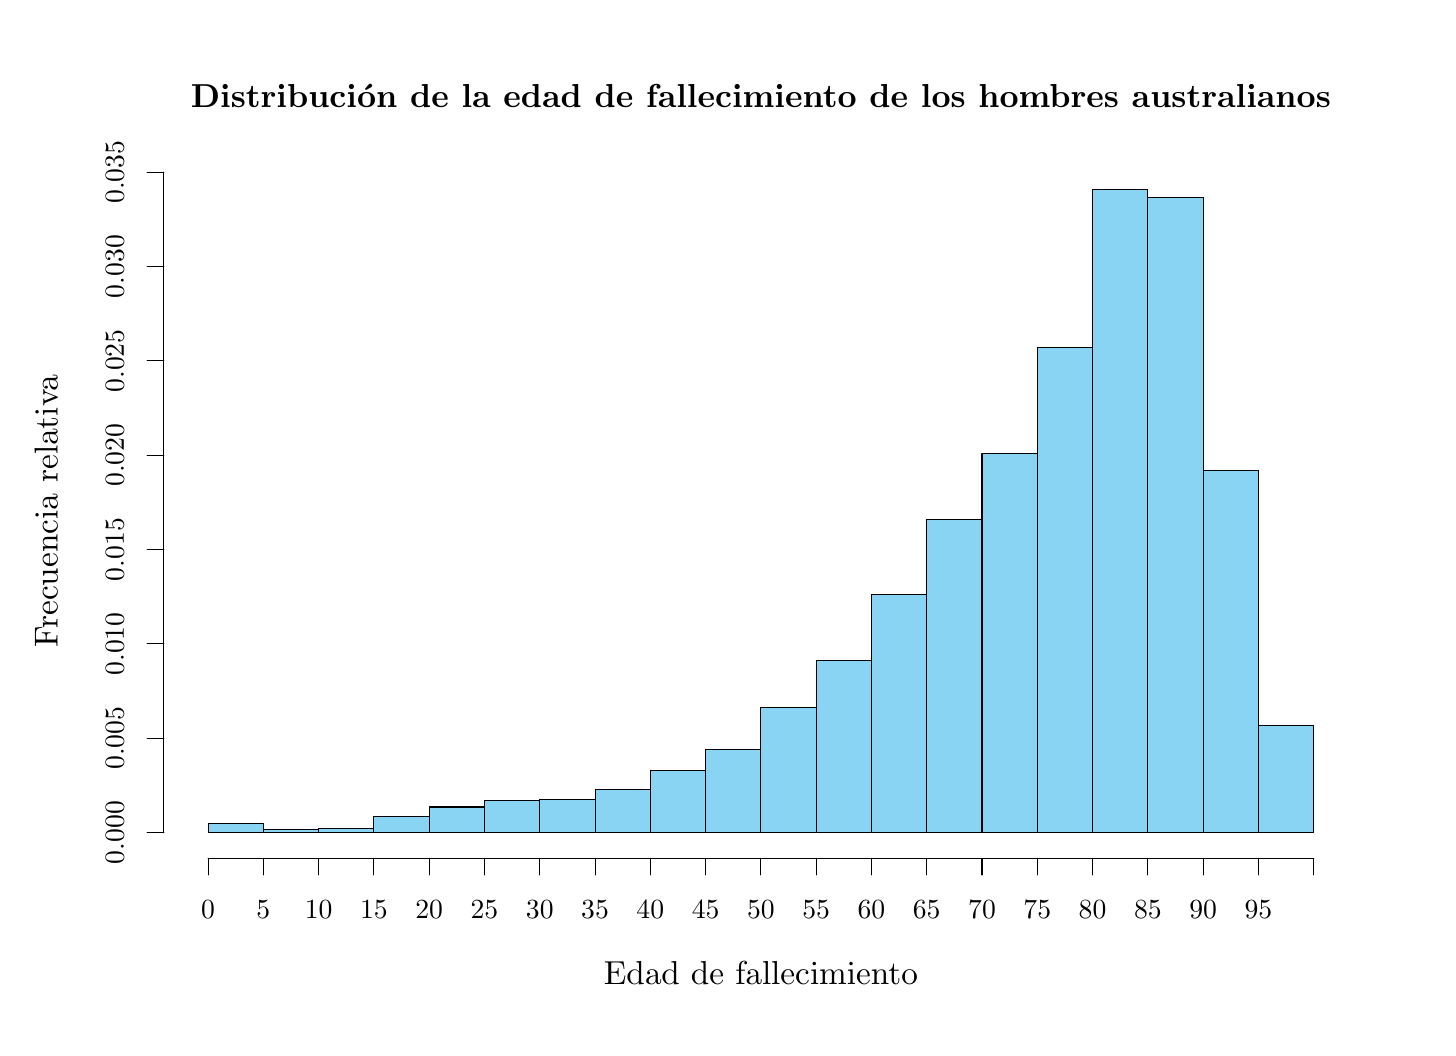
\begin{tikzpicture}[x=1pt,y=1pt]
\definecolor{fillColor}{RGB}{255,255,255}
\path[use as bounding box,fill=fillColor,fill opacity=0.00] (0,0) rectangle (505.89,361.35);
\begin{scope}
\path[clip] (  0.00,  0.00) rectangle (505.89,361.35);
\definecolor{drawColor}{RGB}{0,0,0}

\node[text=drawColor,anchor=base,inner sep=0pt, outer sep=0pt, scale=  1.20] at (264.94,332.61) {\bfseries Distribución de la edad de fallecimiento de los hombres australianos};

\node[text=drawColor,anchor=base,inner sep=0pt, outer sep=0pt, scale=  1.20] at (264.94, 15.60) {Edad de fallecimiento};

\node[text=drawColor,rotate= 90.00,anchor=base,inner sep=0pt, outer sep=0pt, scale=  1.20] at ( 10.80,186.67) {Frecuencia relativa};
\end{scope}
\begin{scope}
\path[clip] (  0.00,  0.00) rectangle (505.89,361.35);
\definecolor{drawColor}{RGB}{0,0,0}

\path[draw=drawColor,line width= 0.4pt,line join=round,line cap=round] ( 49.20, 70.49) -- ( 49.20,309.11);

\path[draw=drawColor,line width= 0.4pt,line join=round,line cap=round] ( 49.20, 70.49) -- ( 43.20, 70.49);

\path[draw=drawColor,line width= 0.4pt,line join=round,line cap=round] ( 49.20,104.58) -- ( 43.20,104.58);

\path[draw=drawColor,line width= 0.4pt,line join=round,line cap=round] ( 49.20,138.67) -- ( 43.20,138.67);

\path[draw=drawColor,line width= 0.4pt,line join=round,line cap=round] ( 49.20,172.76) -- ( 43.20,172.76);

\path[draw=drawColor,line width= 0.4pt,line join=round,line cap=round] ( 49.20,206.85) -- ( 43.20,206.85);

\path[draw=drawColor,line width= 0.4pt,line join=round,line cap=round] ( 49.20,240.94) -- ( 43.20,240.94);

\path[draw=drawColor,line width= 0.4pt,line join=round,line cap=round] ( 49.20,275.03) -- ( 43.20,275.03);

\path[draw=drawColor,line width= 0.4pt,line join=round,line cap=round] ( 49.20,309.11) -- ( 43.20,309.11);

\node[text=drawColor,rotate= 90.00,anchor=base,inner sep=0pt, outer sep=0pt, scale=  1.00] at ( 34.80, 70.49) {0.000};

\node[text=drawColor,rotate= 90.00,anchor=base,inner sep=0pt, outer sep=0pt, scale=  1.00] at ( 34.80,104.58) {0.005};

\node[text=drawColor,rotate= 90.00,anchor=base,inner sep=0pt, outer sep=0pt, scale=  1.00] at ( 34.80,138.67) {0.010};

\node[text=drawColor,rotate= 90.00,anchor=base,inner sep=0pt, outer sep=0pt, scale=  1.00] at ( 34.80,172.76) {0.015};

\node[text=drawColor,rotate= 90.00,anchor=base,inner sep=0pt, outer sep=0pt, scale=  1.00] at ( 34.80,206.85) {0.020};

\node[text=drawColor,rotate= 90.00,anchor=base,inner sep=0pt, outer sep=0pt, scale=  1.00] at ( 34.80,240.94) {0.025};

\node[text=drawColor,rotate= 90.00,anchor=base,inner sep=0pt, outer sep=0pt, scale=  1.00] at ( 34.80,275.03) {0.030};

\node[text=drawColor,rotate= 90.00,anchor=base,inner sep=0pt, outer sep=0pt, scale=  1.00] at ( 34.80,309.11) {0.035};
\end{scope}
\begin{scope}
\path[clip] ( 49.20, 61.20) rectangle (480.69,312.15);
\definecolor{drawColor}{RGB}{0,0,0}
\definecolor{fillColor}{RGB}{137,211,243}

\path[draw=drawColor,line width= 0.4pt,line join=round,line cap=round,fill=fillColor] ( 65.18, 70.49) rectangle ( 85.16, 73.83);

\path[draw=drawColor,line width= 0.4pt,line join=round,line cap=round,fill=fillColor] ( 85.16, 70.49) rectangle (105.13, 71.76);

\path[draw=drawColor,line width= 0.4pt,line join=round,line cap=round,fill=fillColor] (105.13, 70.49) rectangle (125.11, 71.93);

\path[draw=drawColor,line width= 0.4pt,line join=round,line cap=round,fill=fillColor] (125.11, 70.49) rectangle (145.09, 76.37);

\path[draw=drawColor,line width= 0.4pt,line join=round,line cap=round,fill=fillColor] (145.09, 70.49) rectangle (165.06, 79.72);

\path[draw=drawColor,line width= 0.4pt,line join=round,line cap=round,fill=fillColor] (165.06, 70.49) rectangle (185.04, 82.15);

\path[draw=drawColor,line width= 0.4pt,line join=round,line cap=round,fill=fillColor] (185.04, 70.49) rectangle (205.02, 82.56);

\path[draw=drawColor,line width= 0.4pt,line join=round,line cap=round,fill=fillColor] (205.02, 70.49) rectangle (224.99, 86.11);

\path[draw=drawColor,line width= 0.4pt,line join=round,line cap=round,fill=fillColor] (224.99, 70.49) rectangle (244.97, 93.07);

\path[draw=drawColor,line width= 0.4pt,line join=round,line cap=round,fill=fillColor] (244.97, 70.49) rectangle (264.94,100.56);

\path[draw=drawColor,line width= 0.4pt,line join=round,line cap=round,fill=fillColor] (264.94, 70.49) rectangle (284.92,115.77);

\path[draw=drawColor,line width= 0.4pt,line join=round,line cap=round,fill=fillColor] (284.92, 70.49) rectangle (304.90,132.64);

\path[draw=drawColor,line width= 0.4pt,line join=round,line cap=round,fill=fillColor] (304.90, 70.49) rectangle (324.87,156.47);

\path[draw=drawColor,line width= 0.4pt,line join=round,line cap=round,fill=fillColor] (324.87, 70.49) rectangle (344.85,183.77);

\path[draw=drawColor,line width= 0.4pt,line join=round,line cap=round,fill=fillColor] (344.85, 70.49) rectangle (364.83,207.42);

\path[draw=drawColor,line width= 0.4pt,line join=round,line cap=round,fill=fillColor] (364.83, 70.49) rectangle (384.80,245.90);

\path[draw=drawColor,line width= 0.4pt,line join=round,line cap=round,fill=fillColor] (384.80, 70.49) rectangle (404.78,302.86);

\path[draw=drawColor,line width= 0.4pt,line join=round,line cap=round,fill=fillColor] (404.78, 70.49) rectangle (424.76,299.84);

\path[draw=drawColor,line width= 0.4pt,line join=round,line cap=round,fill=fillColor] (424.76, 70.49) rectangle (444.73,201.47);

\path[draw=drawColor,line width= 0.4pt,line join=round,line cap=round,fill=fillColor] (444.73, 70.49) rectangle (464.71,109.24);
\end{scope}
\begin{scope}
\path[clip] (  0.00,  0.00) rectangle (505.89,361.35);
\definecolor{drawColor}{RGB}{0,0,0}

\path[draw=drawColor,line width= 0.4pt,line join=round,line cap=round] ( 65.18, 61.20) -- (464.71, 61.20);

\path[draw=drawColor,line width= 0.4pt,line join=round,line cap=round] ( 65.18, 61.20) -- ( 65.18, 55.20);

\path[draw=drawColor,line width= 0.4pt,line join=round,line cap=round] ( 85.16, 61.20) -- ( 85.16, 55.20);

\path[draw=drawColor,line width= 0.4pt,line join=round,line cap=round] (105.13, 61.20) -- (105.13, 55.20);

\path[draw=drawColor,line width= 0.4pt,line join=round,line cap=round] (125.11, 61.20) -- (125.11, 55.20);

\path[draw=drawColor,line width= 0.4pt,line join=round,line cap=round] (145.09, 61.20) -- (145.09, 55.20);

\path[draw=drawColor,line width= 0.4pt,line join=round,line cap=round] (165.06, 61.20) -- (165.06, 55.20);

\path[draw=drawColor,line width= 0.4pt,line join=round,line cap=round] (185.04, 61.20) -- (185.04, 55.20);

\path[draw=drawColor,line width= 0.4pt,line join=round,line cap=round] (205.02, 61.20) -- (205.02, 55.20);

\path[draw=drawColor,line width= 0.4pt,line join=round,line cap=round] (224.99, 61.20) -- (224.99, 55.20);

\path[draw=drawColor,line width= 0.4pt,line join=round,line cap=round] (244.97, 61.20) -- (244.97, 55.20);

\path[draw=drawColor,line width= 0.4pt,line join=round,line cap=round] (264.94, 61.20) -- (264.94, 55.20);

\path[draw=drawColor,line width= 0.4pt,line join=round,line cap=round] (284.92, 61.20) -- (284.92, 55.20);

\path[draw=drawColor,line width= 0.4pt,line join=round,line cap=round] (304.90, 61.20) -- (304.90, 55.20);

\path[draw=drawColor,line width= 0.4pt,line join=round,line cap=round] (324.87, 61.20) -- (324.87, 55.20);

\path[draw=drawColor,line width= 0.4pt,line join=round,line cap=round] (344.85, 61.20) -- (344.85, 55.20);

\path[draw=drawColor,line width= 0.4pt,line join=round,line cap=round] (364.83, 61.20) -- (364.83, 55.20);

\path[draw=drawColor,line width= 0.4pt,line join=round,line cap=round] (384.80, 61.20) -- (384.80, 55.20);

\path[draw=drawColor,line width= 0.4pt,line join=round,line cap=round] (404.78, 61.20) -- (404.78, 55.20);

\path[draw=drawColor,line width= 0.4pt,line join=round,line cap=round] (424.76, 61.20) -- (424.76, 55.20);

\path[draw=drawColor,line width= 0.4pt,line join=round,line cap=round] (444.73, 61.20) -- (444.73, 55.20);

\path[draw=drawColor,line width= 0.4pt,line join=round,line cap=round] (464.71, 61.20) -- (464.71, 55.20);

\node[text=drawColor,anchor=base,inner sep=0pt, outer sep=0pt, scale=  1.00] at ( 65.18, 39.60) {0};

\node[text=drawColor,anchor=base,inner sep=0pt, outer sep=0pt, scale=  1.00] at ( 85.16, 39.60) {5};

\node[text=drawColor,anchor=base,inner sep=0pt, outer sep=0pt, scale=  1.00] at (105.13, 39.60) {10};

\node[text=drawColor,anchor=base,inner sep=0pt, outer sep=0pt, scale=  1.00] at (125.11, 39.60) {15};

\node[text=drawColor,anchor=base,inner sep=0pt, outer sep=0pt, scale=  1.00] at (145.09, 39.60) {20};

\node[text=drawColor,anchor=base,inner sep=0pt, outer sep=0pt, scale=  1.00] at (165.06, 39.60) {25};

\node[text=drawColor,anchor=base,inner sep=0pt, outer sep=0pt, scale=  1.00] at (185.04, 39.60) {30};

\node[text=drawColor,anchor=base,inner sep=0pt, outer sep=0pt, scale=  1.00] at (205.02, 39.60) {35};

\node[text=drawColor,anchor=base,inner sep=0pt, outer sep=0pt, scale=  1.00] at (224.99, 39.60) {40};

\node[text=drawColor,anchor=base,inner sep=0pt, outer sep=0pt, scale=  1.00] at (244.97, 39.60) {45};

\node[text=drawColor,anchor=base,inner sep=0pt, outer sep=0pt, scale=  1.00] at (264.94, 39.60) {50};

\node[text=drawColor,anchor=base,inner sep=0pt, outer sep=0pt, scale=  1.00] at (284.92, 39.60) {55};

\node[text=drawColor,anchor=base,inner sep=0pt, outer sep=0pt, scale=  1.00] at (304.90, 39.60) {60};

\node[text=drawColor,anchor=base,inner sep=0pt, outer sep=0pt, scale=  1.00] at (324.87, 39.60) {65};

\node[text=drawColor,anchor=base,inner sep=0pt, outer sep=0pt, scale=  1.00] at (344.85, 39.60) {70};

\node[text=drawColor,anchor=base,inner sep=0pt, outer sep=0pt, scale=  1.00] at (364.83, 39.60) {75};

\node[text=drawColor,anchor=base,inner sep=0pt, outer sep=0pt, scale=  1.00] at (384.80, 39.60) {80};

\node[text=drawColor,anchor=base,inner sep=0pt, outer sep=0pt, scale=  1.00] at (404.78, 39.60) {85};

\node[text=drawColor,anchor=base,inner sep=0pt, outer sep=0pt, scale=  1.00] at (424.76, 39.60) {90};

\node[text=drawColor,anchor=base,inner sep=0pt, outer sep=0pt, scale=  1.00] at (444.73, 39.60) {95};
\end{scope}
\end{tikzpicture}
